\documentclass[oneside,14pt,a4paper]{extarticle}
\usepackage[T1,T2A]{fontenc}
\usepackage[a4paper,letterpaper,top=2cm,bottom=2cm,left=2cm,right=1.5cm]{geometry}
\usepackage[utf8]{inputenc}
\usepackage{cmap}
\usepackage[russian,english]{babel}
\usepackage{textcomp}
\usepackage{indentfirst}
\usepackage{graphicx}
\graphicspath{{./}{report/}}
\usepackage{mwe}
\usepackage{wrapfig}
\usepackage{caption}
\usepackage{amsmath}
\usepackage{listings}
\usepackage{amsfonts}
\usepackage{amsthm}
\usepackage[breaklinks]{hyperref}
\usepackage{float}
\usepackage{enumerate, letltxmacro, enumitem}
\usepackage{verbatim, fancyvrb}

\usepackage{titlesec}
\titleformat{\section}{\normalsize\bfseries}{\hspace{1.25cm}\thesection}{1em}{}
\titleformat{\subsection}{\normalsize\bfseries}{\hspace{1.25cm}\thesubsection}{1em}{}
\titleformat{\subsubsection}{\normalsize\bfseries}{\hspace{1.25cm}\thesubsubsection}{1em}{}

\setlength{\parindent}{1.25cm}
\LetLtxMacro\itemold\item
\renewcommand{\item}{\itemindent1.25cm\itemold}
\renewcommand\baselinestretch{1.33}\normalsize
\begin{document}
  \selectlanguage{russian}
  \newpage\thispagestyle{empty}
  
  \begin{center}
      МИНИСТЕРСТВО НАУКИ И ВЫСШЕГО ОБРАЗОВАНИЯ\\
    РОССИЙСКОЙ ФЕДЕРАЦИИ\\
    ФЕДЕРАЛЬНОЕ ГОСУДАРСТВЕННОЕ БЮДЖЕТНОЕ ОБРАЗОВАТЕЛЬНОЕ
    УЧРЕЖДЕНИЕ ВЫСШЕГО ОБРАЗОВАНИЯ\\
    «ВЯТСКИЙ ГОСУДАРСТВЕННЫЙ УНИВЕРСИТЕТ»\\
    Институт математики и информационных систем\\
    Факультет автоматики и вычислительной техники\\
    Кафедра электронных вычислительных машин\\
  \end{center}

  \vfill

  \begin{center}
    Отчет по лабораторной работе № 2\\
    по дисциплине\\
    <<Объектно-ориентированное программирование>>
  \end{center}

  \vfill

  Выполнил студент гр. ИВТб-2301-05-00 \hfill \rule[-0.5mm]{3cm}{0.15mm} /Елпашев С.А./\\[-5ex]

  \begin{tiny}
    \hspace{11cm}(подпись)
  \end{tiny}
  
  Проверил преподаватель \hfill \rule[-0.5mm]{3cm}{0.15mm} /Шмакова Н.А./\\[-5ex]
  
  \begin{tiny}
    \hspace{11cm}(подпись)
  \end{tiny}
  
  \vfill
  
  \begin{center}
    Киров 2026
  \end{center}

  \newpage\thispagestyle{plain}  

  \section{Цель работы}
  Цель работы: изучить и освоить принципы объектно-ориентированного программирования, включая инкапсуляцию, наследование и полиморфизм, путем создания иерархии классов в выбранной предметной области, взаимодействие с базой данных и графическим интерфейсом.

  \section{Задание}
  На основании согласованной в первой лабораторной работе предметной области разработать приложение с  графическим интерфейсом пользователя, используя классы и особенности C\#. Сведения  об объектах предметной области необходимо хранить в БД.

  \section{Решение}
  Проект реализован как ASP.NET Core Web API для управления парком ЭВМ. Предметная область разделена на несколько слоев: модели описывают персональные компьютеры и серверы, контроллер предоставляет HTTP-эндпоинты, сервис содержит бизнес-логику, а контракты и ответы формируют структуру запросов и ответов API.

  Подключение к базе данных реализовано через Entity Framework Core. Основной класс доступа к данным --- \texttt{AppDbContext} из файла \texttt{Data/AppDbContext.cs}. Он наследуется от \texttt{DbContext} и получает в конструкторе объект \\
  \texttt{DbContextOptions<AppDbContext>}, который передается в базовый класс. 

  Добавление контекста производится в \texttt{Program.cs} через метод \texttt{AddDbContext}. В качестве провайдера используется PostgreSQL. Строка подключения берется из конфигурации приложения по ключу \\
  \texttt{ConnectionStrings:Postgres} через \\
  \texttt{builder.Configuration.GetConnectionString("Postgres")}. После запуска приложения контекст извлекается из области видимости зависимостей, и для базы данных вызывается \texttt{Database.EnsureCreated()}, чтобы при отсутствии БД автоматически создать схему.
  
  % EXAMPLE BLOCK START
  Базовый абстрактный класс <<Computer>> содержит:
  \begin{itemize}
    \item[--] Свойства:
    \begin{itemize}
      \item[--] public int Id \{ get; set; \} -- свойство, означающее уникальный идентификатор;
      \item[--] public int ProcessorFrequency \{ get; set; \} -- свойство, означающее частоту процессора в мегагерцах;
      \item[--] public int RamAmount \{ get; set; \} -- свойство, означающее объем оперативной памяти в мегабайтах;
    \end{itemize}
    \item[--] Конструкторы:
    \begin{itemize}
      \item[--] protected Computer() -- защищенный конструктор без параметров;
      \item[--] protected Computer(int processorFrequency) -- защищенный конструктор, принимает частоту процессора и задает объем ОЗУ по умолчанию равным 1024 МБ;
      \item[--] protected Computer(int processorFrequency, int ramAmount) -- защищенный конструктор, принимает частоту процессора и объем оперативной памяти;
    \end{itemize}
    \item[--] Абстрактные методы:
    \begin{itemize}
      \item[--] public abstract string DisplayInfo() -- публичный абстрактный метод, возвращающий информацию об объекте;
      \item[--] public abstract string ExecuteTask() -- публичный абстрактный метод, возвращающий описание выполняемой задачи.
    \end{itemize}
  \end{itemize}

  Класс <<PC>> содержит:
  \begin{itemize}
    \item[--] Свойства:
    \begin{itemize}
      \item[--] public string UserShell \{ get; set; \} -- свойство, означающее пользовательскую оболочку;
      \item[--] public string Os \{ get; set; \} -- свойство, означающее операционную систему;
    \end{itemize}
    \item[--] Конструкторы:
    \begin{itemize}
      \item[--] public PC() : base() -- публичный конструктор без параметров, задает значения по умолчанию;
      \item[--] public PC(int processorFrequency, int ramAmount) : \\
      base(processorFrequency, ramAmount) -- публичный конструктор, принимает частоту процессора и объем ОЗУ;
      \item[--] public PC(int processorFrequency, int ramAmount, string userShell) : base(processorFrequency, ramAmount) -- публичный конструктор, принимает частоту процессора, объем ОЗУ и пользовательскую оболочку;
      \item[--] public PC(int processorFrequency, int ramAmount, string userShell, string os) : base(processorFrequency, ramAmount) -- публичный конструктор, принимает частоту процессора, объем ОЗУ, пользовательскую оболочку и операционную систему;
    \end{itemize}
    \item[--] Методы:
    \begin{itemize}
      \item[--] public void IncreaseRamAmount(int amount) -- публичный метод, увеличивающий объем ОЗУ на заданное значение;
      \item[--] public override string DisplayInfo() -- переопределенный метод, возвращающий информацию о персональном компьютере;
      \item[--] public override string ExecuteTask() -- переопределенный метод, возвращающий описание выполняемой задачи;
      \item[--] public string OpenApplication(string appName) -- публичный метод, возвращающий строку с сообщением об открытии приложения;
      \item[--] public string OpenWebsite(string url) -- публичный метод, возвращающий строку с сообщением об открытии сайта.
    \end{itemize}
  \end{itemize}

  Класс <<Server>> содержит:
  \begin{itemize}
    \item[--] Свойства:
    \begin{itemize}
      \item[--] public int MaxConnections \{ get; set; \} -- свойство, означающее максимальное количество подключений;
      \item[--] public int CurrentConnections \{ get; private set; \} -- свойство, означающее текущее количество подключений;
    \end{itemize}
    \item[--] Конструкторы:
    \begin{itemize}
      \item[--] public Server() : base() -- публичный конструктор без параметров, задает значения по умолчанию;
      \item[--] public Server(int processorFrequency, int ramAmount, int maxConnections) : \\ 
      base(processorFrequency, ramAmount) -- публичный конструктор, принимает частоту процессора, объем ОЗУ и максимальное количество подключений;
      \item[--] public Server(int processorFrequency, int ramAmount, \\ 
      int maxConnections, int currentConnections) : \\
      base(processorFrequency, ramAmount) -- публичный конструктор, принимает частоту процессора, объем ОЗУ, максимальное и текущее количество подключений;
    \end{itemize}
    \item[--] Методы:
    \begin{itemize}
      \item[--] public void Update(int processorFrequency, int ramAmount, \\
      int maxConnections, int currentConnections) -- публичный метод, обновляющий значения основных характеристик сервера;
      \item[--] public void IncrementConnection() -- публичный метод, увеличивающий число активных подключений на единицу;
      \item[--] public override string DisplayInfo() -- переопределенный метод, возвращающий информацию о сервере;
      \item[--] public override string ExecuteTask() -- переопределенный метод, возвращающий описание выполняемой задачи;
  \item[--] public bool AcceptConnection(out string message) -- публичный метод, пытающийся принять новое подключение и возвращающий сообщение о результате;
  \item[--] public string ProcessRequest() -- публичный метод, возвращающий строку с сообщением об обработке сетевого запроса.
    \end{itemize}
  \end{itemize}

  Далее идёт создание контроллера для ответов на запросы для клиентов. Методы для работы с серверами в контроллере реализованы следующим образом:
  \begin{itemize}
    \item[--] public async Task<ActionResult<IEnumerable<ServerSummaryResponse>>> GetAllServers(CancellationToken cancellationToken) -- метод, возвращающий список всех серверов, сохраненных в системе;
    \item[--] public async Task<ActionResult<CreatedResourceResponse>> \\
    CreateServer([FromBody] CreateServerRequest request, CancellationToken \\
    cancellationToken) -- метод, создающий новый сервер, использующий проверку входных данных и метод AddServerAsync для добавления записи в базу данных:
    \begin{Verbatim}[tabsize=4]
      var server = new Server(request.ProcessorFrequency, 
      request.RamAmount, request.MaxConnections, 
      request.CurrentConnections);
      var id = await _computerLabService.AddServerAsync(server, 
      cancellationToken);
    \end{Verbatim}
    \item[--] public async Task<ActionResult<ServerSummaryResponse>> \\
    UpdateServer([FromRoute] int id, [FromBody] CreateServerRequest request, \\
    CancellationToken cancellationToken) -- метод, обновляющий существующий сервер по уникальному идентификатору;
    \item[--] public async Task<IActionResult> DeleteServer([FromRoute] int id, \\
    CancellationToken cancellationToken) -- метод, удаляющий сервер по уникальному идентификатору;
    \item[--] public async Task<ActionResult<OperationMessageResponse>> \\
    GetServerInfo([FromRoute] int id, CancellationToken cancellationToken) -- метод, возвращающий полное описание сервера по уникальному идентификатору, используя метод DisplayInfo();
    \item[--] public async Task<ActionResult<OperationMessageResponse>> \\
    ExecuteServerTask([FromRoute] int id, CancellationToken cancellationToken) -- метод, возвращающий описание выполняемой сервером задачи, используя метод ExecuteTask();
    \item[--] public async Task<ActionResult<ConnectionStatusResponse>> \\
    AcceptServerConnection([FromRoute] int id, CancellationToken cancellationToken) -- метод, принимающий новое подключение к серверу и возвращающий сообщение о результате, используя метод AcceptConnection();
    \item[--] public async Task<ActionResult<OperationMessageResponse>> \\
    ProcessServerRequest([FromRoute] int id, CancellationToken cancellationToken) -- метод, возвращающий сообщение об обработке сетевого запроса, используя метод ProcessRequest().
  \end{itemize}

  Для компьютеров сделано всё по аналогии.

  Диаграмма классов проекта представлена на рисунке 1.

  \begin{figure}[H]
    \centering
    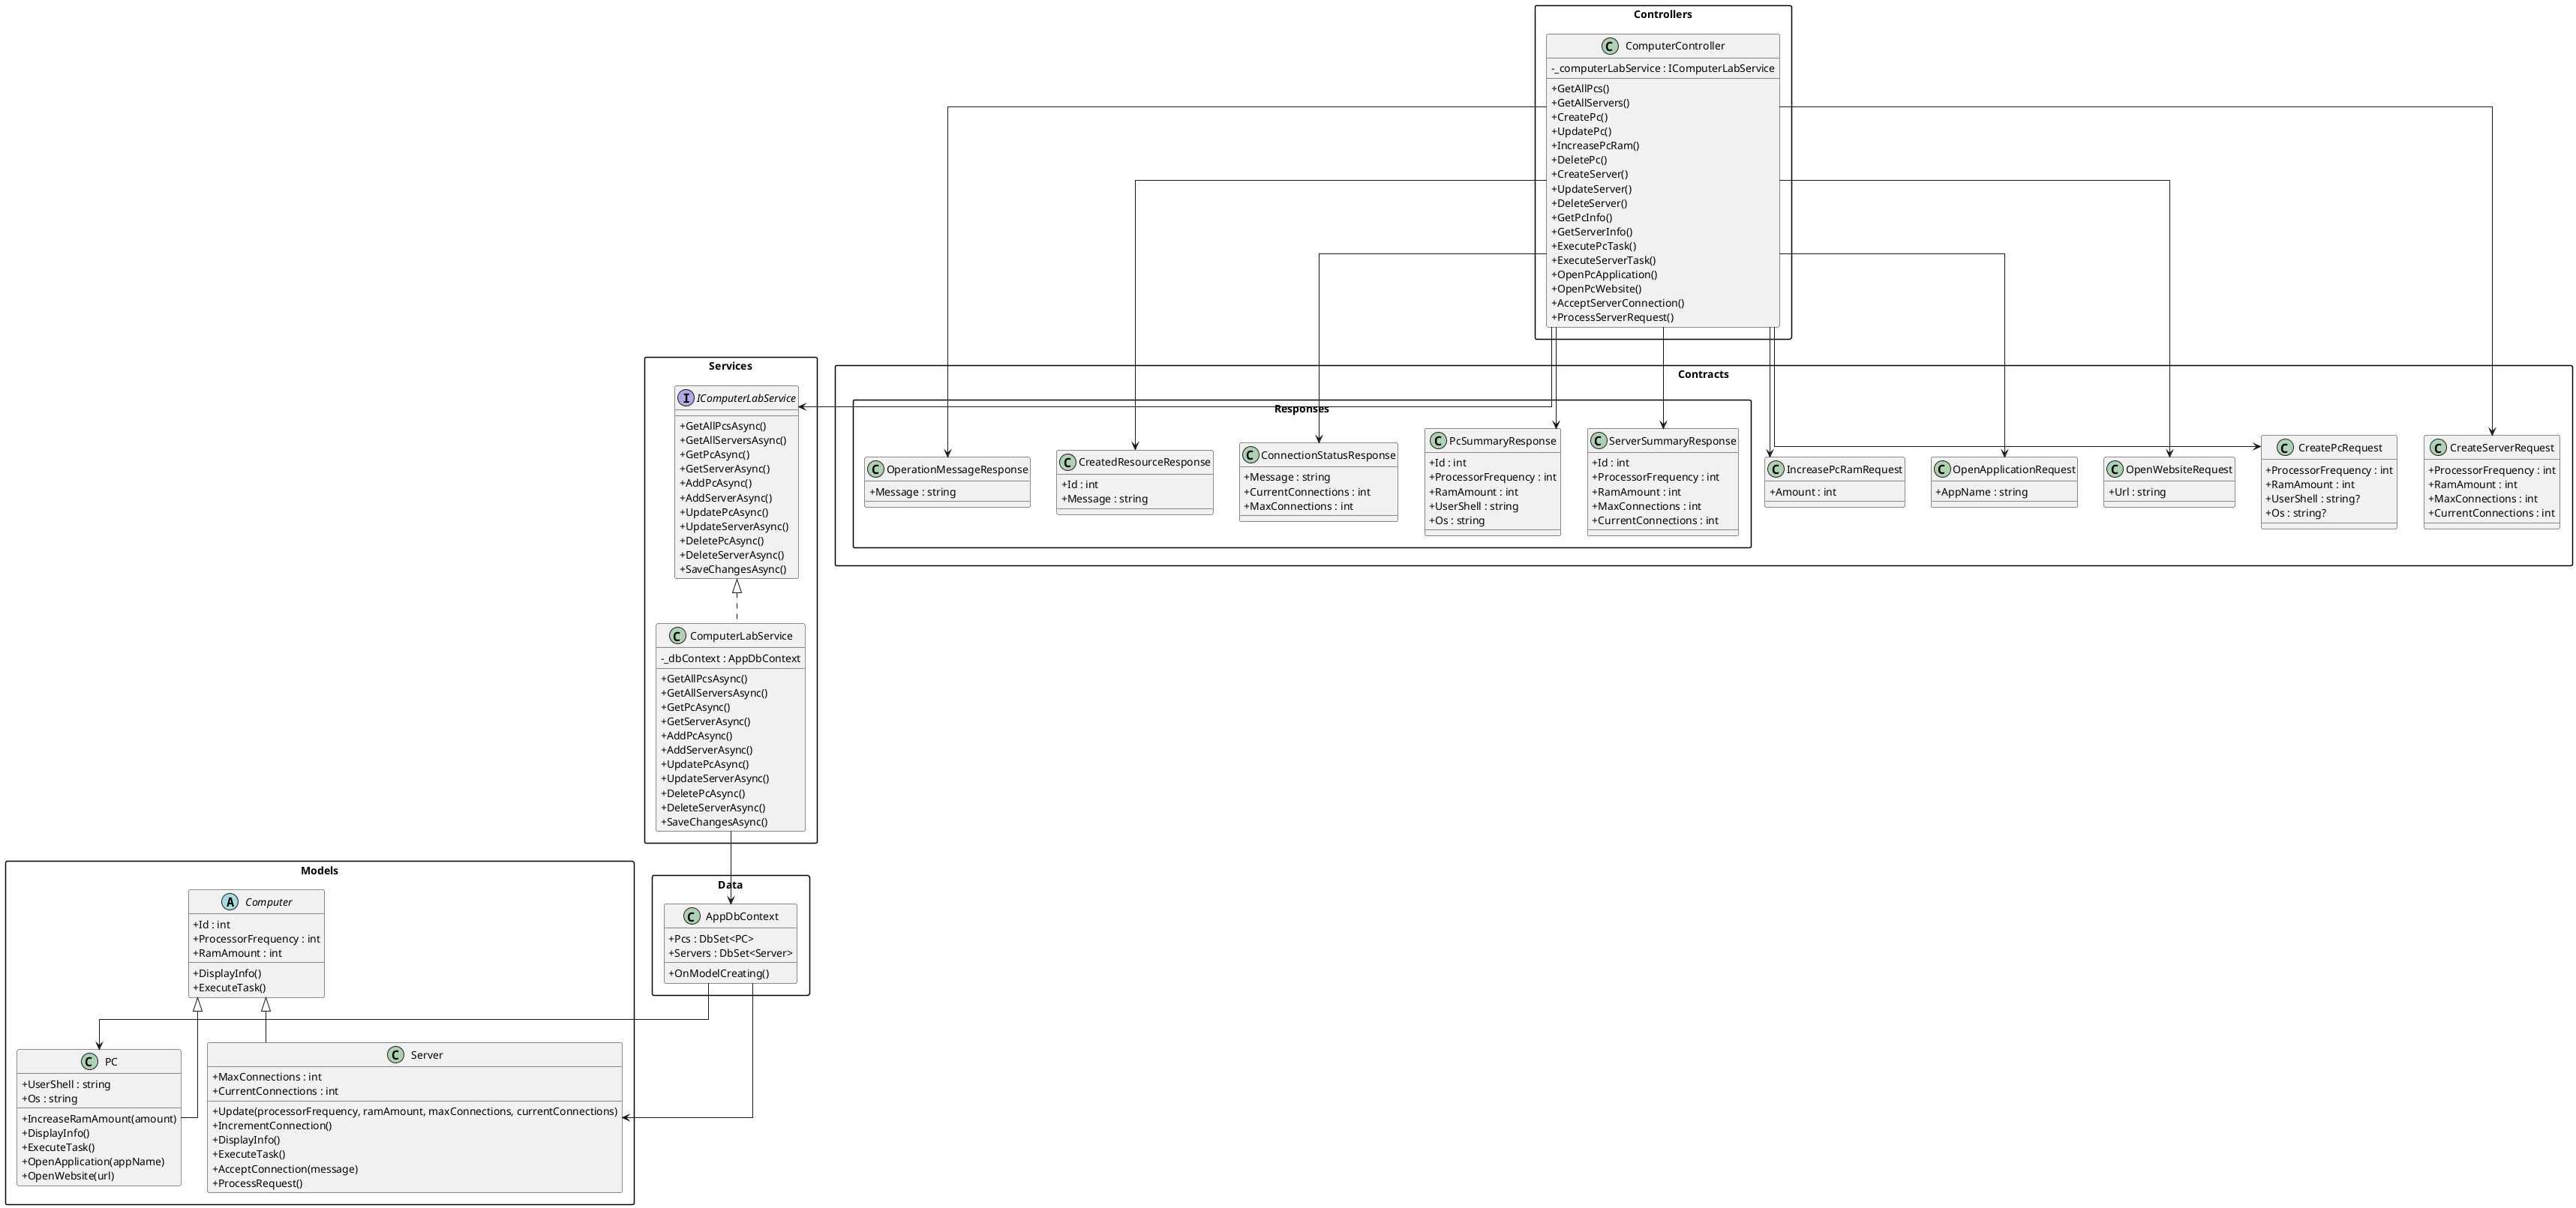
\includegraphics[width=\textwidth]{class_d.png}
    \caption{Диаграмма классов проекта}
  \end{figure}

  \section{Скриншоты работы программы}
  

  \begin{figure}[H]
    \centering
    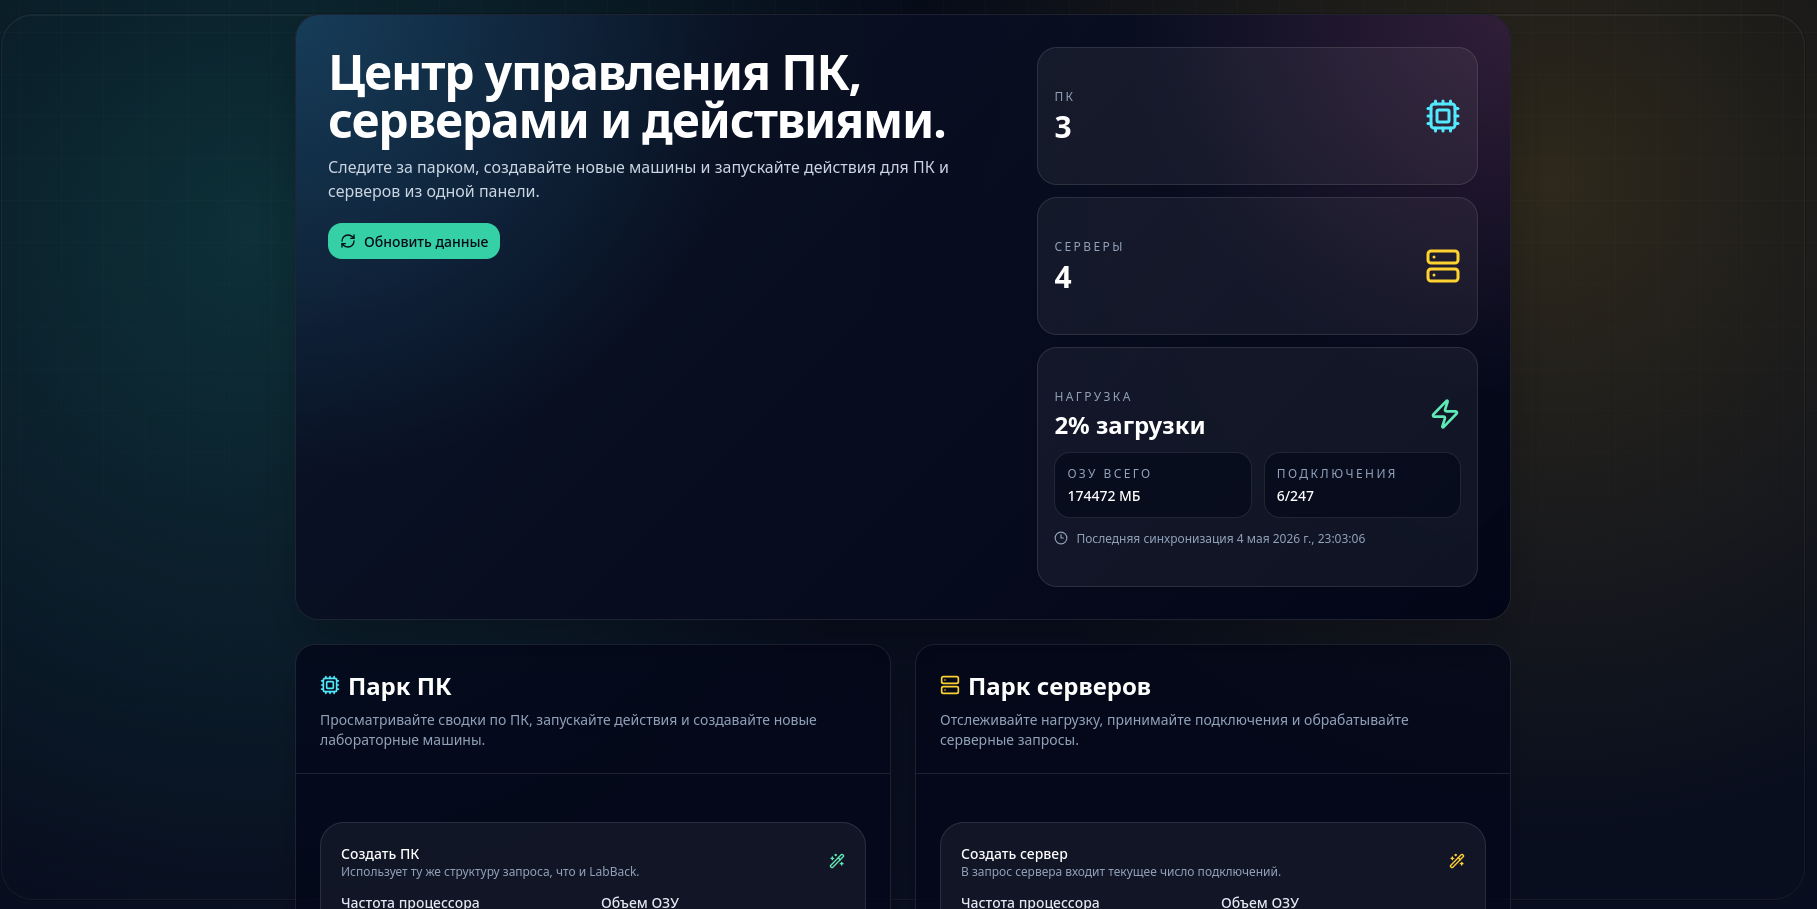
\includegraphics[width=\textwidth]{./main.png}
    \caption{Главный экран сайта}
  \end{figure}

  \begin{figure}[H]
    \centering
    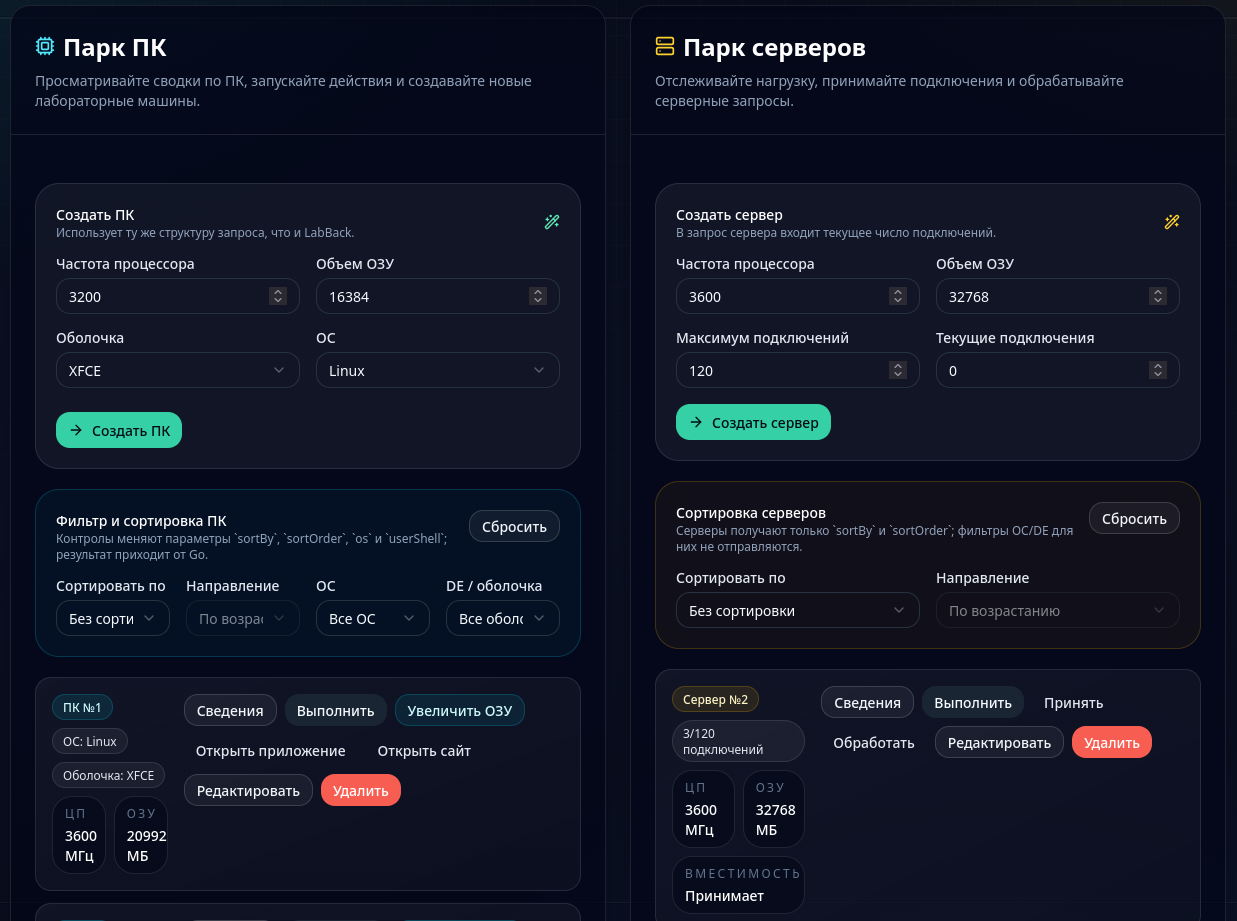
\includegraphics[width=\textwidth]{./list.png}
    \caption{Список серверов и компьютеров}
  \end{figure}

  \begin{figure}[H]
    \centering
    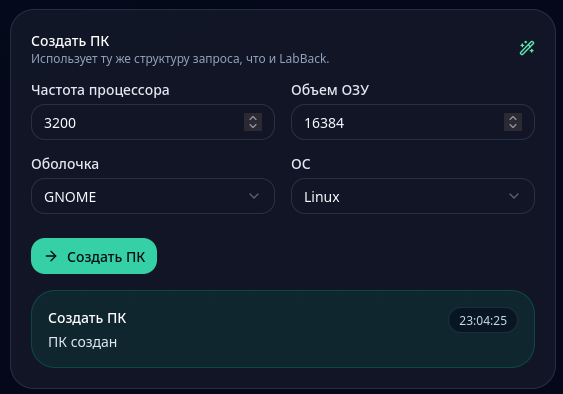
\includegraphics[width=\textwidth]{./notif.png}
    \caption{Вывод сообщения о добавлении}
  \end{figure}


  \begin{figure}[H]
    \centering
    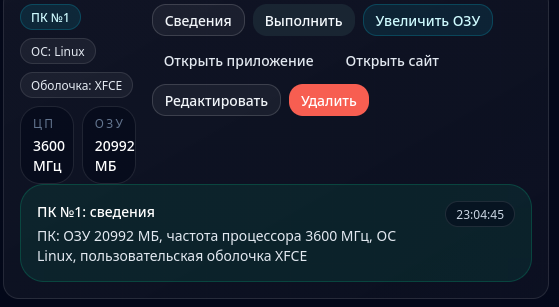
\includegraphics[width=\textwidth]{./info.png}
    \caption{Вывод информации об объекте}
  \end{figure}

  Исходный код выполненной лабораторной работы представлен в текущем репозитории проекта -- . 

  \newpage\thispagestyle{plain}
  \section{Вывод}
  В ходе выполнения лабораторной работы была разработана и реализована иерархия классов и сопутствующая инфраструктура Web API для управления парком ЭВМ. Изучены основные принципы объектно-ориентированного программирования: инкапсуляция, наследование и полиморфизм. Разработано приложение, демонстрирующее применение данных принципов на уровне доменной модели, контроллера и слоя доступа к данным.
\end{document}
